\documentclass[10pt]{article}
\usepackage{cacs2026}
\usepackage{amsmath}
\let\Bbbk\relax % cacs2026.sty's newtxmath already defines \Bbbk; amssymb redefining it is a known conflict
\usepackage{amssymb}
\usepackage{xcolor}
\usepackage{multirow}
\usepackage{algorithm}
\usepackage{algorithmic}
\usepackage{tikz}
\usetikzlibrary{arrows.meta,positioning,fit,backgrounds}
\usepackage{float} % [H] to pin Fig. 5 exactly under its preceding paragraph, not float elsewhere
% cacs2026.sty's own caption config names figures "Figure" (name=Figure),
% but the template's own written instructions ("Use the abbreviation
% 'Fig. 1'") and every in-text reference in this paper use "Fig." --
% overriding just the label text here, not any other caption styling,
% to make the printed caption match both.
\captionsetup[figure]{name=Fig.}
% Categorical palette shared with the dataviz-validated result plots
% (experiments/plots/common.py's ARM_STYLE), reused for Fig. 2 (the
% testbed architecture schematic).
\definecolor{palBlue}{HTML}{2A78D6}
\definecolor{palGreen}{HTML}{008300}
\definecolor{palYellow}{HTML}{EDA100}
\definecolor{palPurple}{HTML}{7A5CD6}

% Separate, non-overlapping palette for Fig. 1 (the methodology
% pipeline) only, deliberately distinct hues from the palette above,
% so the two schematics are never confused with one another.
\definecolor{palTeal}{HTML}{157F7F}
\definecolor{palRust}{HTML}{C1502E}
\definecolor{palPlum}{HTML}{8E3B6B}

% Visible TODO marker for content the author (not Claude) writes.
\newcommand{\authorTODO}[1]{\par\noindent\fbox{\parbox{0.95\linewidth}{\textbf{\color{red}TODO(MANOJ):} #1}}\par}

% Float/caption spacing is prescribed by cacs2026.sty itself, so it is
% not overridden here, matching the official template's own instruction
% not to alter margins/spacing.

% article's default float-placement limits (topfraction=0.7, topnumber=2,
% totalnumber=3) are too tight for this section's cluster of one table +
% three figures declared close together: LaTeX defers floats past those
% limits onto their own column instead of the same column as the text
% discussing them, leaving that column mostly-float and the facing one
% empty. Loosening only the placement fractions/counts, not any spacing
% cacs2026.sty itself sets.
\renewcommand{\topfraction}{0.95}
\renewcommand{\textfraction}{0.05}
\renewcommand{\floatpagefraction}{0.8}
\setcounter{topnumber}{4}
\setcounter{totalnumber}{6}

\begin{document}

\CACSmaketitle
  {DQN-QoE Slice Admission Control for Live OAI Open RAN}
  {Manoj Prasad Kunasegran, Wai Leong Pang\textsuperscript{*}, and Swee King Phang}

\begin{CACSabstract}
\abstractnameCACS
Slice Admission Control (SAC) decides whether an incoming slice request can be accommodated given
current resources. However, static SAC cannot adapt as user demands shift, particularly in dynamic 5G environments.
Deep Reinforcement Learning (DRL)-driven SAC closes
this gap by incorporating context-aware mechanisms such as Service Level Agreement (SLA) and Quality of Experience (QoE) into the admission policy. We evaluate a Deep Q-Network (DQN)-based approach on a real OpenAirInterface (OAI)
gNodeB across three slices, namely Enhanced Mobile Broadband
(eMBB), Ultra-Reliable Low-Latency Communication (URLLC) and Massive
Machine-Type Communication (mMTC). The QoE-aware policy is
benchmarked against a static baseline, an SLA-only reward,
and a static-at-cap policy that pins every slice at its calibrated
maximum allocation. After finalising QoE calibration, a
fully powered live evaluation across 128 episodes per arm demonstrated
the QoE-aware DQN sustaining 100.0\% eMBB/URLLC/mMTC SLA compliance
on every episode, a statistically significant improvement over the
static baseline's 93.9\% slice-wide compliance. The SLA-only reward
and the static-at-cap policy converge to a statistically
indistinguishable compliance rate, 98.6\% and 98.7\% slice-wide
respectively. Five further SLA-reward checkpoints
show that live robustness also varies substantially despite
equivalent offline convergence. Under a congested,
URLLC-preservation scenario, the DQN policy trades eMBB compliance
for URLLC compliance offline. However, during live evaluation, every arm remains fully
SLA-compliant. A smaller pilot still shows the QoE-aware reward
giving URLLC a materially higher Mean Opinion Score of 4.83 out of
5, against 2.44 for the SLA-only reward and 2.66 for the static
baseline. Negligible control-loop latency of 0.57\,ms and a
lightweight model under 20,000 parameters confirm minimal deployment
overhead. These findings demonstrate the feasibility of deploying DRL-driven SAC in a live Open RAN architecture.
\end{CACSabstract}

\begin{center}
\parbox{0.94\columnwidth}{\fontsize{9}{10.5}\selectfont\noindent
\textit{Index Terms}---5G, Deep Reinforcement Learning, Network Slicing, Open RAN, Quality of Experience, Slice Admission Control}
\end{center}

\CACSfirstpagefootnote{%
M.~P.~Kunasegran, W.~L.~Pang, and S.~K.~Phang are with the School of
Engineering, Taylor's University, Subang Jaya, Malaysia.\\
\textsuperscript{*}Corresponding author.\\
ORCID: M.~P.~Kunasegran, 0009-0005-3169-1873; W.~L.~Pang,
0000-0001-8407-5648; S.~K.~Phang, 0000-0002-7877-8766.}

\section{Introduction and Background}
Network slicing virtualises physical 5G deployments to serve
heterogeneous classes under per-slice Service Level Agreements
(SLAs). Ultra-Reliable Low-Latency Communication (URLLC) needs
sub-millisecond latency, Enhanced Mobile Broadband (eMBB) needs high
throughput, and Massive Machine-Type Communication (mMTC) serves
many low-power devices. Slice Admission Control (SAC) decides whether
an incoming request can be accommodated given current resources, and
static SAC cannot adapt effectively as user demand changes over time.

Our prior work applied DRL to SAC under gNodeB (gNB) congestion, using
SLA-driven reward shaping to prioritise URLLC traffic
\cite{mecon-paper1}. It later expanded to a third slice type, mMTC,
with load balancing across multiple gNBs \cite{icraie-paper2}. Both
were validated only in simulation. Our systematic review
\cite{survey-paper3} places this research space into three evidence
tiers. These are literature-supported work, preliminary simulated
studies and a proposed but not-yet-validated graph-attention
multi-agent federated-learning (GAT-MARL-FL) framework, identifying validated deployment as a gap.
This paper closes that gap for the same formulation. We realise it on
a real OpenAirInterface (OAI) gNB over its native E2 interface, the
O-RAN near-real-time RAN Intelligent Controller (RIC)
\cite{oran-e2ap}. Only the radio channel remains simulated, a mode we
denote '\textit{rfsim}' throughout, and the reward is centred on QoE rather than
SLA compliance alone. This paper makes the following
contributions:
\begin{enumerate}[itemsep=1pt,topsep=2pt,parsep=0pt,partopsep=0pt]
\item We deploy a DRL-based SAC policy on a real O-RAN E2 control
loop and identify a structural difference from existing work
\cite{mecon-paper1,icraie-paper2}. Only a per-slice resource ceiling
is exposed, not a per-flow accept/reject primitive, so admission is
realised as a ceiling adjustment.
\item We show that a QoE-aware reward significantly outperforms the
SLA-only reward of \cite{mecon-paper1,icraie-paper2} and a
static-at-cap arm on the same live O-RAN, with negligible
control-loop overhead.
\item We evaluate a congested scenario offline and, at a smaller
scale, live. This shows where the offline scarcity mechanism does
and does not carry over to a deployed O-RAN.
\item This single-agent, single-gNB deployment validates the live
control loop that the multi-agent GAT-MARL-FL framework in
\cite{survey-paper3} would incorporate in future work.
\end{enumerate}

\section{Literature Review}
This section reviews ten QoE-focused works from the verified pool of
\cite{survey-paper3}. Recent DRL-driven slicing work has moved from SLA/QoS objectives
toward explicit QoE. The authors in \cite{wang2025usercentric} used a
hierarchical dueling DQN for user-centric bandwidth allocation,
maximising satisfaction under stochastic requests while lowering
latency. The researchers in \cite{lai2024multiresource} termed their
formulation DRL-MQS, for multi-resource QoS satisfaction, reporting a
10.5\% improvement in QoS-satisfaction ratio. Another study
\cite{kougioumtzidis2025drlvr} trained a multi-agent Deep
Deterministic Policy Gradient (DDPG) model for transmission-level QoE
in wireless Virtual Reality (VR) over 5G New Radio (NR). The authors
in \cite{chen2026qoeslicing} combined Convolutional Neural
Network-Long Short-Term Memory (CNN-LSTM) prediction with
Lyapunov-stable, non-DRL QoE-aware allocation. Another paper
\cite{yin2026qoestin} instead used multi-agent Proximal Policy
Optimisation (PPO), or MAPPO, for QoE across satellite-terrestrial
Multi-access Edge Computing (MEC) services. All five studies remain
simulation-only.

A parallel thread infers QoE from network-side signals. The authors
in \cite{sun2025qoeric} used a Transformer encoder-decoder to predict
real-time-video QoE from low-level RAN information, cutting Mean
Absolute Error (MAE) by $12.5$--$44\%$. Meanwhile, \cite{gonzalez2025qoeoran}
embedded a gradient-boosting QoE estimator in a 5G O-RAN, reaching a
coefficient of determination $R^2=0.986$. Both remain estimation only.

Closest to the present setting, three works place QoE control inside
the O-RAN loop, none deploying a learned admission policy over
a live E2 loop. The authors in \cite{anand2024qoexapp} classified
users by interference via an ML-based xApp, raising R-Factor scores in a simulated 5G HetNet.
The researchers in \cite{casparsen2025vroran} demonstrated
near-real-time xApp RAN slicing, an open-loop Radio Resource
Management (RRM) policy on an OAI plus FlexRIC testbed. FlexRIC is an
open-source O-RAN near-real-time RIC. This work cuts overprovisioning
by 30\% and is the only one reviewed here validated on a live O-RAN,
though unlearned. Meanwhile, \cite{yeznabad2024clqdba} proposed a
cross-layer QoE-driven bitrate heuristic for MEC video in simulation.

Across this literature, QoE is emerging as the primary objective and
DRL the dominant method, yet none of the ten works reviewed here
deploy a learned QoE-aware admission policy over a live E2 loop.
Closing that gap is the central objective of this paper.

\section{Methodology}
This section describes the testbed and admission-control problem
formulation, summarised by Fig.~\ref{fig:pipeline}, with no new
algorithmic framework proposed at this stage. Offline
training against a closed-loop simulator, detailed in
Section~\ref{sec:offline-env}, produces frozen checkpoints. These
deploy on the live testbed below with no further learning, and any
checkpoint failing offline convergence is discarded first. A held-out
offline evaluation runs alongside this pipeline but does not
rank-correlate with live outcomes.

\begin{figure}[t]
\centering
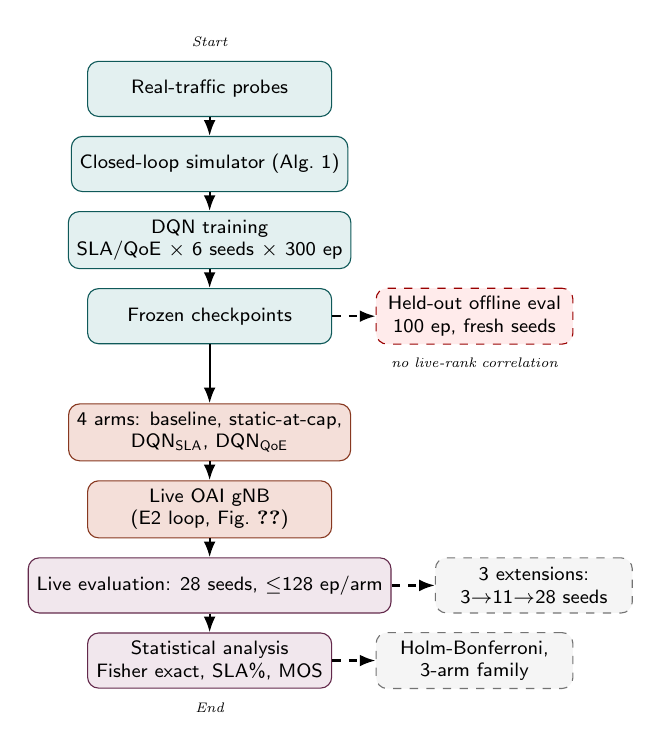
\begin{tikzpicture}[
  font=\sffamily\scriptsize,
  box/.style={draw, rounded corners, align=center, inner sep=3pt, minimum height=0.7cm, minimum width=3.1cm},
  simbox/.style={box, fill=palTeal!12, draw=palTeal!70!black},
  livebox/.style={box, fill=palRust!18, draw=palRust!70!black},
  evalbox/.style={box, fill=palPlum!12, draw=palPlum!70!black},
  warnbox/.style={box, fill=red!8, draw=red!60!black, dashed, minimum width=2.5cm},
  infobox/.style={box, fill=black!4, draw=black!55, dashed, minimum width=2.5cm},
  arrow/.style={-{Latex[length=2mm]}, thick},
  dashedarrow/.style={-{Latex[length=2mm]}, thick, dashed},
]
\node[simbox] (probe) {Real-traffic probes};
\node[font=\tiny\itshape, above=0.06cm of probe] {Start};
\node[simbox, below=0.24cm of probe] (sim) {Closed-loop simulator (Alg.~1)};
\node[simbox, below=0.24cm of sim] (train) {DQN training\\SLA/QoE $\times$ 6 seeds $\times$ 300 ep};
\node[simbox, below=0.24cm of train] (ckpt) {Frozen checkpoints};
\node[livebox, below=0.75cm of ckpt] (arms) {4 arms: baseline, static-at-cap,\\DQN$_{\text{SLA}}$, DQN$_{\text{QoE}}$};
\node[livebox, below=0.24cm of arms] (rig) {Live OAI gNB\\(E2 loop, Fig.~\ref{fig:architecture})};
\node[evalbox, below=0.24cm of rig] (liveeval) {Live evaluation: 28 seeds, $\leq$128 ep/arm};
\node[evalbox, below=0.24cm of liveeval] (stats) {Statistical analysis\\Fisher exact, SLA\%, MOS};
\node[font=\tiny\itshape, below=0.06cm of stats] {End};

\draw[arrow] (probe) -- (sim);
\draw[arrow] (sim) -- (train);
\draw[arrow] (train) -- (ckpt);
\draw[arrow] (ckpt) -- (arms);
\draw[arrow] (arms) -- (rig);
\draw[arrow] (rig) -- (liveeval);
\draw[arrow] (liveeval) -- (stats);

\node[warnbox, right=0.55cm of ckpt] (offeval) {Held-out offline eval\\100 ep, fresh seeds};
\draw[dashedarrow] (ckpt.east) -- (offeval.west);
\node[font=\tiny\itshape, below=0.04cm of offeval, align=center, text width=3.0cm] {no live-rank correlation};

\node[infobox, right=0.55cm of liveeval] (liveinfo) {3 extensions:\\3$\to$11$\to$28 seeds};
\draw[dashedarrow] (liveeval.east) -- (liveinfo.west);

\node[infobox, right=0.55cm of stats] (statsinfo) {Holm-Bonferroni,\\3-arm family};
\draw[dashedarrow] (stats.east) -- (statsinfo.west);
\end{tikzpicture}
\caption{End-to-end methodology, frozen checkpoints deployed live with no further learning, summarised in Table~\ref{tab:results} and Figs.~\ref{fig:compliance-a}--\ref{fig:compliance-b}.}
\label{fig:pipeline}
\end{figure}

\subsection{Testbed}
\begin{figure*}[t]
\centering
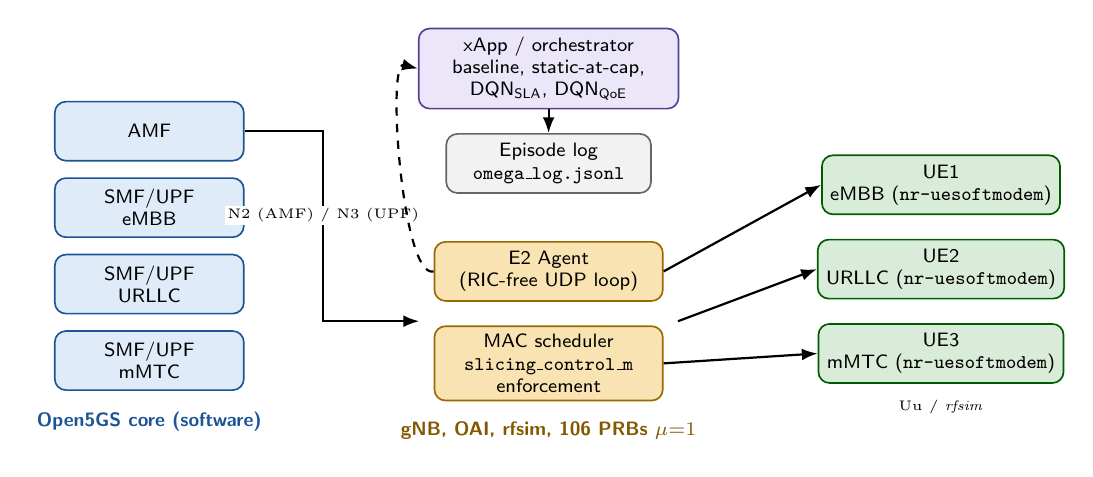
\begin{tikzpicture}[
  font=\sffamily\scriptsize,
  box/.style={draw, rounded corners, minimum height=0.75cm, align=center, inner sep=3pt, line width=0.6pt},
  core/.style={box, fill=palBlue!15, draw=palBlue!70!black},
  gnb/.style={box, fill=palYellow!30, draw=palYellow!65!black},
  ue/.style={box, fill=palGreen!15, draw=palGreen!70!black, minimum width=2.0cm},
  xapp/.style={box, fill=palPurple!15, draw=palPurple!70!black},
  logbox/.style={box, fill=black!5, draw=black!60, minimum width=2.6cm},
  arrow/.style={-{Latex[length=2mm]}, thick},
  dashedarrow/.style={-{Latex[length=2mm]}, thick, dashed},
]
\node[core, minimum width=2.4cm] (amf) {AMF};
\node[core, minimum width=2.4cm, below=0.2cm of amf] (smf1) {SMF/UPF\\eMBB};
\node[core, minimum width=2.4cm, below=0.2cm of smf1] (smf2) {SMF/UPF\\URLLC};
\node[core, minimum width=2.4cm, below=0.2cm of smf2] (smf3) {SMF/UPF\\mMTC};
\node[font=\sffamily\bfseries\scriptsize, text=palBlue!70!black, below=0.14cm of smf3] (coretitle) {Open5GS core (software)};

\node[xapp, minimum width=3.3cm, right=2.2cm of smf1.north east, anchor=north west, yshift=1.9cm] (xapp) {xApp / orchestrator\\baseline, static-at-cap,\\DQN$_{\text{SLA}}$, DQN$_{\text{QoE}}$};
\node[logbox, below=0.3cm of xapp] (log) {Episode log\\\texttt{omega\_log.jsonl}};

\node[gnb, minimum width=2.9cm, below=0.6cm of log] (e2) {E2 Agent\\(RIC-free UDP loop)};
\node[gnb, minimum width=2.9cm, below=0.3cm of e2] (mac) {MAC scheduler\\\texttt{slicing\_control\_m}\\enforcement};
\node[font=\sffamily\bfseries\scriptsize, text=palYellow!55!black, below=0.14cm of mac] (gnbtitle) {gNB, OAI, \textit{rfsim}, 106 PRBs $\mu{=}1$};
\node[fit=(mac)(e2), inner sep=5pt] (gnbbox) {};

\node[ue, right=2.0cm of e2, yshift=1.1cm] (ue1) {UE1\\eMBB (\texttt{nr-uesoftmodem})};
\node[ue, below=0.3cm of ue1] (ue2) {UE2\\URLLC (\texttt{nr-uesoftmodem})};
\node[ue, below=0.3cm of ue2] (ue3) {UE3\\mMTC (\texttt{nr-uesoftmodem})};

\draw[arrow] (amf.east) -- ++(1.0,0) coordinate (n2n3) -- (n2n3 |- gnbbox.west) node[midway, above, font=\tiny, fill=white, inner sep=1pt] {N2 (AMF) / N3 (UPF)} -- (gnbbox.west);
\draw[arrow] (e2.east) -- (ue1.west);
\draw[arrow] (gnbbox.east) -- (ue2.west);
\draw[arrow] (mac.east) -- (ue3.west);
\node[font=\tiny, below=0.08cm of ue3] {Uu / \textit{rfsim}};
\draw[dashedarrow] (e2.west) .. controls +(-0.4,-0.1) and +(-0.4,0.1) .. (xapp.west);
\draw[arrow] (xapp) -- (log);
\end{tikzpicture}
\caption{Testbed software architecture.}
\label{fig:architecture}
\end{figure*}

Fig.~\ref{fig:architecture} shows the Open5GS core connecting over
N2/N3, carrying signalling to the Access and Mobility Management
Function (AMF) and data to the User Plane Function (UPF). Both reach
a real OAI gNB, an ORANSlice fork \cite{oranslice} with a simulated
radio channel, \textit{rfsim}. Its nominal capacity is 106 Physical Resource
Blocks (PRBs) at $\mu=1$, and its Medium Access Control (MAC)
scheduler enforces the per-slice ceiling. Three
\texttt{nr-uesoftmodem} UEs, one per slice, attach over the radio
interface. The RIC-free E2
agent exchanges User Datagram Protocol (UDP) INDICATION/RESPONSE and
CONTROL messages with the xApp/orchestrator, shared by all four arms.
These messages carry \texttt{sst}, \texttt{sd}, \texttt{min\_ratio}
and \texttt{max\_ratio}. Every step is logged to
\texttt{omega\_log.jsonl}.

Unlike the earlier simulated formulation \cite{mecon-paper1,icraie-paper2},
the real O-RAN E2 interface exposes only a per-slice ratio ceiling on
a 0--100 scale rather than a binary accept/reject action
\cite{oran-e2ap}. An accept decision raises a slice's ceiling toward
a calibrated maximum, and a reject lowers it toward a floor. Ceiling
values were calibrated by direct measurement, since the scale maps
nonlinearly onto real PRBs here. The static baseline holds its
ceiling fixed for the whole episode. \emph{Static-at-cap} instead pins every
ceiling at its calibrated maximum from the start, testing whether a
generous fixed allocation alone matches a learned policy. Learned
arms are DQN policies \cite{dqn}, all four issuing decisions through
the same E2 agent/xApp loop.

\subsection{Problem Formulation}
\label{sec:problem-formulation}
The gNB state at time $t$ is defined as
\begin{equation}
s_t = \left(\frac{U_s(t)}{B}, \; C_t, \; \frac{L_s(t)}{L_{\max}} \;\forall s \in \mathcal{S}\right),
\label{eq:state}
\end{equation}
where $U_s(t)$ is the resource allocation of slice $s \in
\mathcal{S}=\{\text{eMBB},\text{URLLC},\text{mMTC}\}$ and $B$ is the
total resource budget on the ceiling's 0--100 scale. $C_t$ is the
current congestion level, and $L_s(t)$ is slice $s$'s queue length
normalised by its capacity $L_{\max}$. The agent's action at each
step is the ceiling adjustment described above. The SLA-only reward,
used to train DQN-SLA, is
\begin{equation}
r(s_t,a_t) = \sum_{s\in\mathcal{S}}\big(\omega_s R_s - \lambda_s\big) - \mu C_t\|a_t\|_1,
\label{eq:reward}
\end{equation}
where $\omega_s$ and $\lambda_s$ are slice $s$'s reward weight and
SLA-violation penalty, and $R_s$ is the reward for serving slice $s$.
The term $\mu C_t\|a_t\|_1$ penalises total accepted volume by
congestion level, matching existing work's SLA-driven reward
structure \cite{mecon-paper1,icraie-paper2}. DQN-QoE instead trains
against a differently-shaped reward, our own prior work's eq.\,(9)
\cite{survey-paper3}, not an additive extension of Eq.~\eqref{eq:reward}.
{\setlength{\abovedisplayskip}{5pt plus 1pt minus 1pt}%
\setlength{\belowdisplayskip}{5pt plus 1pt minus 1pt}%
\setlength{\abovedisplayshortskip}{3pt plus 1pt minus 1pt}%
\setlength{\belowdisplayshortskip}{3pt plus 1pt minus 1pt}%
\begin{equation}
r^{\mathrm{QoE}}(s_t,a_t) = \kappa\,\overline{\mathrm{MOS}}_t - \nu\,\mathrm{cost}_t - \theta\,\mathrm{viol}_t,
\label{eq:qoe-reward}
\end{equation}
where $\overline{\mathrm{MOS}}_t\in[0,1]$ rescales the mean per-slice
Mean Opinion Score (MOS) from Eqs.~\eqref{eq:iqx-arg}--\eqref{eq:iqx},
\begin{equation}
q_t = \max\big(\gamma\,\ell_t + \delta\,p_t + \epsilon/\tau_t,\ 0\big),
\label{eq:iqx-arg}
\end{equation}
\begin{equation}
\mathrm{MOS}_t = \mathrm{clip}\big(\alpha - \beta\log(1+q_t),\ 1,\ 5\big).
\label{eq:iqx}
\end{equation}}
$\ell_t,p_t,\tau_t$ are latency, packet loss and throughput.
$\alpha,\beta,\gamma,\delta,\epsilon$ are coefficients calibrated in
Section~\ref{sec:feasibility}. Above, $\mathrm{cost}_t$ reuses
Eq.~\eqref{eq:reward}'s congestion-scaled accepted volume
$\mu C_t\|a_t\|_1$. The term $\mathrm{viol}_t$ is the mean per-slice
violation severity, continuous unlike $\lambda_s$'s flat charge. We
compare both variants on the same live setup. We also
report a priority-weighted compliance score $W =
\sum_{s\in\mathcal{S}} \pi_s\,\mathrm{Compl}_s$, in place of an
unweighted average. Here $\mathrm{Compl}_s$ is slice $s$'s
fully-compliant-episode rate, and $\pi_s = \omega_s$ is the same
reward weight from Eq.~\eqref{eq:reward}, normalised so
$\sum_s \pi_s=1$.

\subsection{Offline Training Environment}
\label{sec:offline-env}
A DQN policy needs hundreds of episodes per seed to converge, 1,800
across this study's six checkpoints alone, far more live rig time
than this paper's entire live evaluation uses. Training therefore
happens offline, against a synthetic, closed-loop source. Served
traffic is capped by the slice's most recent ceiling, and unserved
demand persists as backlog. An admission decision therefore carries a
real, delayed consequence, unlike an earlier open-loop source where
always accepting was trivially reward-optimal. Algorithm~\ref{alg:sim}
summarises the closed-loop update, one polling step per gNB/slice
pair.

\begin{algorithm}[t]
\caption{Offline closed-loop 5G traffic simulation (one polling step, all gNBs/slices)}
\label{alg:sim}
\footnotesize
\begin{algorithmic}[1]
\REQUIRE per-(gNB,slice) state: offered, backlog, ceiling, UE set
\FORALL{gNB $g$, slice $s$}
  \STATE $mean \gets$ mean\_offered\_ratio$_s \times B \times$ gnb\_load$_g$
  \STATE offered$_{g,s} \gets \max(0,\ \text{offered}_{g,s} + 0.1(mean - \text{offered}_{g,s}) + \text{noise})$
  \IF{a reject freed backlog on the previous step}
    \STATE backlog$_{g,s} \gets \max(0,\ \text{backlog}_{g,s} - \text{relief})$
  \ENDIF
  \STATE $demand \gets \text{offered}_{g,s} + \text{backlog}_{g,s}$
  \STATE $served \gets \min(demand,\ \text{ceiling}_{g,s})$
  \STATE backlog$_{g,s} \gets \min(\text{backlog\_cap},\ demand - served)$
  \STATE with prob.\ churn\_prob, replace one UE's RNTI in $(g,s)$
  \STATE $bler \gets 0.02 + 0.3 \times (\text{backlog}_{g,s} / \text{backlog\_cap})$
  \FORALL{UE $u$ in $(g,s)$'s set, $n \gets |\text{UEs}_{g,s}|$}
    \STATE emit KPM sample for $u$: $served/n$, $bler$, backlog$_{g,s}/n$
  \ENDFOR
\ENDFOR
\STATE agent observes the resulting state $s_t$
\STATE agent sends ceiling$_{g,s}\ \forall (g,s)$ for the next step
\end{algorithmic}
\end{algorithm}

This source's demand mean is tied to offered-load levels measured on
this rig, but its temporal dynamics are not validated against live
traffic. Held-out evaluation of the
same six checkpoints does not rank-correlate with live compliance.
This traces in part to the
simulator's backlog-capacity parameter, which was never validated
against real SLA-margin magnitude. Offline training still produces competent policies but
cannot rank or pre-select which checkpoint will succeed live, so
every number in this paper's Results is a live measurement, not
an offline projection.

\subsection{Evaluation Setup}
Each of the four arms was evaluated live across 28 random seeds, with
frozen policy weights, reached in three extensions. The first added 3
seeds at 2 episodes each. The second added 8 more at the full
5-episode protocol, once a QoE-calibration issue detailed in
Section~\ref{sec:feasibility} was corrected, for a running total of
46 episodes/arm. The third added 17
more, 16 at 5 episodes and one at 2, for the fully powered 128
episodes/arm reported here. This sample is large enough that a tied
Fisher exact test is genuine, not underpowered. The static-at-cap arm reuses the
static baseline's control code with only the ceiling changed. The
DQN arms followed the offline training procedure, 300 episodes per seed.

\section{Results and Discussion}
\subsection{Live Testbed Results}
\label{sec:live-results}
We classify a live episode as \emph{fully compliant} if every
per-step SLA margin stays positive for all three slices, and
\emph{collapsed} otherwise. Each margin is sampled every 5 seconds
and taken as whichever of queue-occupancy or packet-loss is worse.
Table~\ref{tab:results}
summarises SLA compliance for all four arms across 128 live episodes
each, under the corrected QoE calibration from
Section~\ref{sec:feasibility}. DQN-QoE sustains 100\% compliance on
every slice, every episode, 128 of 128. DQN-SLA and
static-at-cap reach an identical, slightly lower 126/128. The
static baseline trails both at 120/128, its ceiling staying flat
rather than rising toward the calibrated maximum.

\begin{table}[t]
\centering
\caption{Live SLA compliance (\%), 128 episodes/arm}
\label{tab:results}
\small
\begin{tabular}{@{}lrrr@{}}
\toprule
Arm & eMBB & URLLC & mMTC \\
\midrule
Static & 94.0 & 93.8 & 93.9 \\
Static-at-cap & 99.1 & 98.4 & 98.5 \\
DQN (SLA reward) & 98.8 & 98.4 & 98.5 \\
DQN (QoE reward) & \textbf{100.0} & \textbf{100.0} & \textbf{100.0} \\
\bottomrule
\end{tabular}
\end{table}

Fig.~\ref{fig:sla-vs-qoe-ceiling} plots DQN-QoE against DQN-SLA on
the one seed where DQN-SLA collapses. Between steps 33--36, it drops
URLLC's ceiling as low as half its cap before recovering, while
DQN-QoE holds cap throughout. This is the mechanism behind that
episode's 0\% vs.\ 100\% URLLC outcome, raising whether DQN's
advantage reduces to a more generous fixed ceiling. An earlier,
smaller-sample evaluation suggested static-at-cap collapses more
often than DQN-SLA. The gap was 27\% vs.\ 0\%, $p=0.0149$. At
this paper's $3\times$ larger sample, that edge does not hold. Both
reach an identical 126/128, $p=1.0$, a genuine null result. Both
separate further from the baseline's 120/128 than at 46 episodes/arm,
but only DQN-QoE's gap is significant. Raw $p=0.10$ for DQN-SLA and
static-at-cap vs.\ baseline, identical at 126/128 each, and
$p=0.0070$ for DQN-QoE vs.\ baseline become $p=0.205$ and
$p=0.021$ after correction. The QoE-aware reward's advantage
survives correction, but the SLA-only reward's does not.

\begin{figure}[t]
\centering
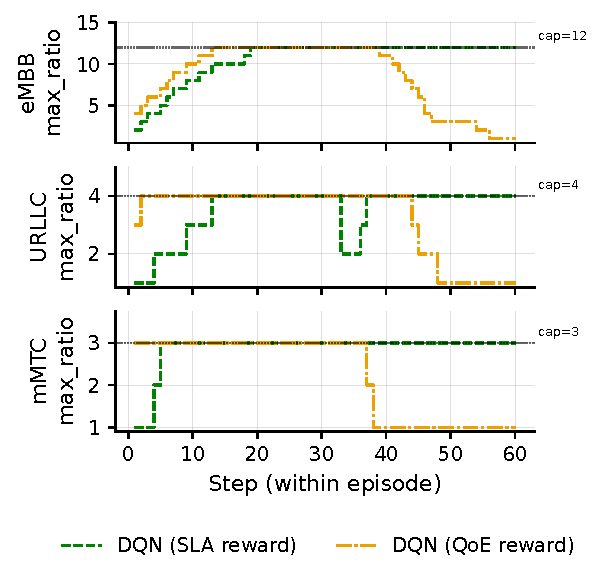
\includegraphics[width=0.98\linewidth]{figures/fig_sla_vs_qoe_ceiling.pdf}
\caption{Commanded ceiling per slice, DQN-SLA vs.\ DQN-QoE, seed 955, episode 1.}
\label{fig:sla-vs-qoe-ceiling}
\end{figure}

Fig.~\ref{fig:compliance-a} shows this episode-by-episode, one point
per episode, DQN-QoE at 100\% throughout and the other three in the
same bimodal split. Fig.~\ref{fig:compliance-b} shows two bars per
arm, only DQN-QoE's coinciding at 100\%. We also trained 5 more DQN-SLA checkpoints at a reduced 21-episode
protocol. Despite indistinguishable offline convergence, live records
varied substantially. Of the five, 3 were perfect and one reached
19/21. The remaining checkpoint fell to 13/21, worse than baseline.
This observation confirms that live
robustness is not
predictable from offline convergence alone, as
Section~\ref{sec:offline-env} details.

\begin{figure}[t]
\centering
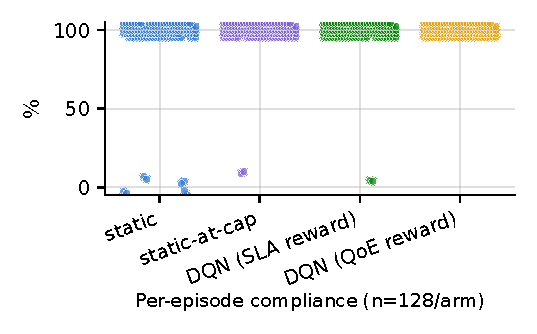
\includegraphics[width=0.98\linewidth]{figures/fig2_sla_compliance_a.pdf}
\caption{Per-episode SLA compliance (\%), one point per episode.}
\label{fig:compliance-a}
\end{figure}

\begin{table}[t]
\centering
\caption{Congested offline compliance (\%), pooled 165 ep/arm}
\label{tab:congested}
\footnotesize
\begin{tabular}{@{}lrrrr@{}}
\toprule
Arm & URLLC & eMBB & mMTC & $W$ \\
\midrule
Static baseline & 19.7 & 32.7 & 19.8 & \textbf{24.9} \\
DQN (SLA reward) & 27.7 & 7.7 & 9.4 & 19.1 \\
DQN (QoE reward) & 25.0 & 8.2 & 11.6 & 17.9 \\
\bottomrule
\end{tabular}
\end{table}

\subsection{Deployment Feasibility}
\label{sec:feasibility}
Measured against the real gNB, the E2 round trip has a median latency
of 0.57\,ms. Its 90th/99th percentiles, the worst 10\%/1\% of
calls, reach 1.10\,ms and 1.77\,ms. The DQN model, 18,562 parameters
and $\sim$300\,KB on disk, selects an action with a median CPU
inference latency of 67.9--68.3\,$\mu$s. p90/p99 reach
84.6--85.1/108.9--115.0\,$\mu$s across both reward modes, a small
fraction of the 5-second control interval. The step's actual dominant cost is
the QoE-mapper Long Short-Term Memory (LSTM) inference at $\sim$7.3\,ms, an order of magnitude
above the DQN decision at $\sim$0.07\,ms or the E2 exchange at
$\sim$0.6\,ms, all three staying under 2\% of the step
budget. The configured 5.0\,s control cadence lands at 5000.7\,ms, a
0.7\,ms gap. Comparing offline predictions against live
results showed a good match for eMBB but not URLLC/mMTC, trained
under a different demand assumption than observed live, and surfaced
a QoE-calibration bug. The MOS estimator's throughput term used a
PRB-usage ratio at run time, but eMBB's coefficients assumed an
absolute per-UE PRB count. This meant 0.15 read as almost-starved,
pinning eMBB's MOS at the scale floor. Refitting
those coefficients against the ratio actually used lifted eMBB's MOS
from a uniform 1.00 to 2.29, 3.62, and 4.11. This predates
Table~\ref{tab:results}, unaffected by the MOS estimate.

\subsection{Congested Scenario, Offline Results and a Live Pilot}
Unlike the constant demand of Sections~\ref{sec:live-results}
and~\ref{sec:feasibility}, we evaluate the same checkpoints
against a congested extension of Section~\ref{sec:offline-env}'s
offline source, where demand exceeding the shared pool scales down
each slice's allocation proportionally. Pooled over 165 held-out
episodes/arm across 11 seeds, Table~\ref{tab:congested}
shows both DQN variants raising URLLC compliance above the baseline.
Both trade off eMBB and mMTC compliance, matching existing work's
URLLC-first behaviour \cite{mecon-paper1,icraie-paper2}. Applying
$W$, with $\omega_{\mathrm{URLLC}}=5.0$ and $\omega_{\mathrm{eMBB}}=3.5$,
the baseline still scores higher overall. URLLC carries the larger
weight, but the DQN arms gain only 5--8 points of URLLC compliance
against a 24--25 point eMBB loss, so eMBB's larger raw swing
outweighs URLLC's smaller weighted gain. We also live-evaluated the
same checkpoints at a smaller pilot scale, one seed and two episodes
per arm. Every arm was fully SLA-compliant live, a scale mismatch
since this rig's ceilings never approach the offline budget's
contention. The QoE-aware reward still produced a
materially higher URLLC MOS of 4.83 out of 5 than the SLA-only
reward's 2.44 or the static baseline's 2.66, at the same 100\%
compliance.

\begin{figure}[H]
\centering
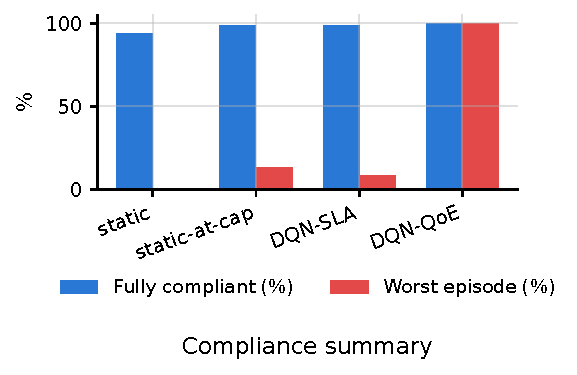
\includegraphics[width=0.98\linewidth]{figures/fig2_sla_compliance_b.pdf}
\caption{Compliance summary, fraction of episodes fully SLA-compliant and worst single-episode compliance, by arm.}
\label{fig:compliance-b}
\end{figure}

\section{Conclusion and Future Work}
This paper moved an existing simulated DRL-based SAC formulation
onto a real OAI gNB over its native E2 control loop, with the radio
channel still simulated. A fully powered live evaluation across 128
episodes per arm confirmed the QoE-aware reward's significant
compliance advantage over the static baseline, 100.0\% against
93.9\% slice-wide. It is the only arm whose gain over baseline
survives Holm-Bonferroni correction, $p=0.021$. The SLA-only reward
and static-at-cap policy reach 98.6\% and 98.7\%, numerically ahead
of the baseline but not significant after correction, $p=0.205$.
Control-loop overhead stayed negligible throughout. Median E2
round-trip latency was 0.57\,ms and DQN inference
67.9--68.3\,$\mu$s, several orders of magnitude below the 5\,s
control cadence, from a model under 20,000 parameters. Under offline
congestion, the learned policy prioritises URLLC unless priorities
are weighted through $W$. No live arm faced that tradeoff at this
rig's contention level. The QoE-aware reward still gave URLLC a
materially higher experience score, MOS 4.83 against 2.44--2.66, at
matched compliance.

Our future work will improve the offline environment's fidelity to
real traffic. In particular, the closed-loop simulator's
backlog-capacity parameter needs validating against measured live
SLA-margin magnitude rather than offered-load levels alone, since
held-out evaluation of the same checkpoints does not rank-correlate
with live compliance. We will also extend this deployment toward the
fully-fledged GAT-MARL-FL framework from our earlier review. This
single-agent, single-gNB deployment leaves open whether the E2
interface's per-slice ceiling primitive still suffices once a
graph-attention policy coordinates multiple gNBs, and whether the
negligible control-loop overhead measured here holds once
coordination and federated aggregation run on top of it. This leaves
topology-scalability, federated-learning privacy and
disruption-resilience open.

\componentheading{Acknowledgment}
This research was supported by the Ministry of Higher Education
(MOHE), Malaysia through the Fundamental Research Grant Scheme
(FRGS/1/2024/ICT06/TAYLOR/02/1).

\enlargethispage{4\baselineskip}
\bibliographystyle{IEEEtran}
\bibliography{refs}

\end{document}
